% Options for packages loaded elsewhere
\PassOptionsToPackage{unicode}{hyperref}
\PassOptionsToPackage{hyphens}{url}
%
\documentclass[
]{article}
\usepackage{lmodern}
\usepackage{amssymb,amsmath}
\usepackage{ifxetex,ifluatex}
\ifnum 0\ifxetex 1\fi\ifluatex 1\fi=0 % if pdftex
  \usepackage[T1]{fontenc}
  \usepackage[utf8]{inputenc}
  \usepackage{textcomp} % provide euro and other symbols
\else % if luatex or xetex
  \usepackage{unicode-math}
  \defaultfontfeatures{Scale=MatchLowercase}
  \defaultfontfeatures[\rmfamily]{Ligatures=TeX,Scale=1}
\fi
% Use upquote if available, for straight quotes in verbatim environments
\IfFileExists{upquote.sty}{\usepackage{upquote}}{}
\IfFileExists{microtype.sty}{% use microtype if available
  \usepackage[]{microtype}
  \UseMicrotypeSet[protrusion]{basicmath} % disable protrusion for tt fonts
}{}
\makeatletter
\@ifundefined{KOMAClassName}{% if non-KOMA class
  \IfFileExists{parskip.sty}{%
    \usepackage{parskip}
  }{% else
    \setlength{\parindent}{0pt}
    \setlength{\parskip}{6pt plus 2pt minus 1pt}}
}{% if KOMA class
  \KOMAoptions{parskip=half}}
\makeatother
\usepackage{xcolor}
\IfFileExists{xurl.sty}{\usepackage{xurl}}{} % add URL line breaks if available
\IfFileExists{bookmark.sty}{\usepackage{bookmark}}{\usepackage{hyperref}}
\hypersetup{
  pdftitle={Metodos De Ordenamiento Simple},
  pdfauthor={Geremias Baudino},
  hidelinks,
  pdfcreator={LaTeX via pandoc}}
\urlstyle{same} % disable monospaced font for URLs
\usepackage[margin=1in]{geometry}
\usepackage{color}
\usepackage{fancyvrb}
\newcommand{\VerbBar}{|}
\newcommand{\VERB}{\Verb[commandchars=\\\{\}]}
\DefineVerbatimEnvironment{Highlighting}{Verbatim}{commandchars=\\\{\}}
% Add ',fontsize=\small' for more characters per line
\usepackage{framed}
\definecolor{shadecolor}{RGB}{248,248,248}
\newenvironment{Shaded}{\begin{snugshade}}{\end{snugshade}}
\newcommand{\AlertTok}[1]{\textcolor[rgb]{0.94,0.16,0.16}{#1}}
\newcommand{\AnnotationTok}[1]{\textcolor[rgb]{0.56,0.35,0.01}{\textbf{\textit{#1}}}}
\newcommand{\AttributeTok}[1]{\textcolor[rgb]{0.77,0.63,0.00}{#1}}
\newcommand{\BaseNTok}[1]{\textcolor[rgb]{0.00,0.00,0.81}{#1}}
\newcommand{\BuiltInTok}[1]{#1}
\newcommand{\CharTok}[1]{\textcolor[rgb]{0.31,0.60,0.02}{#1}}
\newcommand{\CommentTok}[1]{\textcolor[rgb]{0.56,0.35,0.01}{\textit{#1}}}
\newcommand{\CommentVarTok}[1]{\textcolor[rgb]{0.56,0.35,0.01}{\textbf{\textit{#1}}}}
\newcommand{\ConstantTok}[1]{\textcolor[rgb]{0.00,0.00,0.00}{#1}}
\newcommand{\ControlFlowTok}[1]{\textcolor[rgb]{0.13,0.29,0.53}{\textbf{#1}}}
\newcommand{\DataTypeTok}[1]{\textcolor[rgb]{0.13,0.29,0.53}{#1}}
\newcommand{\DecValTok}[1]{\textcolor[rgb]{0.00,0.00,0.81}{#1}}
\newcommand{\DocumentationTok}[1]{\textcolor[rgb]{0.56,0.35,0.01}{\textbf{\textit{#1}}}}
\newcommand{\ErrorTok}[1]{\textcolor[rgb]{0.64,0.00,0.00}{\textbf{#1}}}
\newcommand{\ExtensionTok}[1]{#1}
\newcommand{\FloatTok}[1]{\textcolor[rgb]{0.00,0.00,0.81}{#1}}
\newcommand{\FunctionTok}[1]{\textcolor[rgb]{0.00,0.00,0.00}{#1}}
\newcommand{\ImportTok}[1]{#1}
\newcommand{\InformationTok}[1]{\textcolor[rgb]{0.56,0.35,0.01}{\textbf{\textit{#1}}}}
\newcommand{\KeywordTok}[1]{\textcolor[rgb]{0.13,0.29,0.53}{\textbf{#1}}}
\newcommand{\NormalTok}[1]{#1}
\newcommand{\OperatorTok}[1]{\textcolor[rgb]{0.81,0.36,0.00}{\textbf{#1}}}
\newcommand{\OtherTok}[1]{\textcolor[rgb]{0.56,0.35,0.01}{#1}}
\newcommand{\PreprocessorTok}[1]{\textcolor[rgb]{0.56,0.35,0.01}{\textit{#1}}}
\newcommand{\RegionMarkerTok}[1]{#1}
\newcommand{\SpecialCharTok}[1]{\textcolor[rgb]{0.00,0.00,0.00}{#1}}
\newcommand{\SpecialStringTok}[1]{\textcolor[rgb]{0.31,0.60,0.02}{#1}}
\newcommand{\StringTok}[1]{\textcolor[rgb]{0.31,0.60,0.02}{#1}}
\newcommand{\VariableTok}[1]{\textcolor[rgb]{0.00,0.00,0.00}{#1}}
\newcommand{\VerbatimStringTok}[1]{\textcolor[rgb]{0.31,0.60,0.02}{#1}}
\newcommand{\WarningTok}[1]{\textcolor[rgb]{0.56,0.35,0.01}{\textbf{\textit{#1}}}}
\usepackage{graphicx,grffile}
\makeatletter
\def\maxwidth{\ifdim\Gin@nat@width>\linewidth\linewidth\else\Gin@nat@width\fi}
\def\maxheight{\ifdim\Gin@nat@height>\textheight\textheight\else\Gin@nat@height\fi}
\makeatother
% Scale images if necessary, so that they will not overflow the page
% margins by default, and it is still possible to overwrite the defaults
% using explicit options in \includegraphics[width, height, ...]{}
\setkeys{Gin}{width=\maxwidth,height=\maxheight,keepaspectratio}
% Set default figure placement to htbp
\makeatletter
\def\fps@figure{htbp}
\makeatother
\setlength{\emergencystretch}{3em} % prevent overfull lines
\providecommand{\tightlist}{%
  \setlength{\itemsep}{0pt}\setlength{\parskip}{0pt}}
\setcounter{secnumdepth}{-\maxdimen} % remove section numbering

\title{Metodos De Ordenamiento Simple}
\author{Geremias Baudino}
\date{10/10/2020}

\begin{document}
\maketitle

\hypertarget{metodos-de-ordenamiento-iterativo}{%
\subsubsection{1 - Metodos de Ordenamiento
Iterativo}\label{metodos-de-ordenamiento-iterativo}}

Los metodos de ordenamiento iterativo son aquellos que se realizan de
forma que el codigo deba de repetirse una y otra vez hasta comprobar que
ha sido ordenado por completo.

\hypertarget{metodo-de-ordenamiento-de-la-burbuja-bubblesort}{%
\paragraph{1.1 - Metodo de Ordenamiento de la Burbuja
(BubbleSort)}\label{metodo-de-ordenamiento-de-la-burbuja-bubblesort}}

El Ordenamiento de burbuja (BubbleSort) es un algoritmo de ordenamiento
simple. El mismo funciona revisando cada elemento de la lista a ordenar
con el que le sigue, cambiándolos de posición si están en un orden
incorrecto (n\textgreater n+1). Es necesario repetir este proceso varias
veces hasta que no se necesiten más cambios, lo que significa que la
lista quedó ordenada.

Su código en Python 3 sería el siguiente:

\begin{Shaded}
\begin{Highlighting}[]
\ImportTok{from}\NormalTok{ random }\ImportTok{import}\NormalTok{ sample }\CommentTok{# Importamos un metodo de la biblioteca random para generar listas aleatorias}
\NormalTok{lista }\OperatorTok{=} \BuiltInTok{list}\NormalTok{(}\BuiltInTok{range}\NormalTok{(}\DecValTok{100}\NormalTok{)) }\CommentTok{# Creamos la lista base con números del 1 al 100}

\CommentTok{# Creamos una lista aleatoria con la func sample (contiene 5 elementos aleatorios de la lista base)}
\NormalTok{vectorbs }\OperatorTok{=}\NormalTok{ sample(lista,}\DecValTok{5}\NormalTok{) }


\KeywordTok{def}\NormalTok{ bubblesort(vectorbs):}
    \CommentTok{"""Esta función ordenara el vector que le pases como argumento con el metodo de Bubble Sort"""}
    
    \CommentTok{# Imprimimos la lista obtenida al principio (Desordenada)}
    \BuiltInTok{print}\NormalTok{(}\StringTok{"El vector a ordenar es: "}\NormalTok{,vectorbs)}
\NormalTok{    n }\OperatorTok{=} \DecValTok{0} \CommentTok{# Establecemos un contador del largo del vector}
    
    \ControlFlowTok{for}\NormalTok{ _ }\KeywordTok{in}\NormalTok{ vectorbs:}
\NormalTok{        n }\OperatorTok{+=} \DecValTok{1} \CommentTok{#Contamos la cantidad de caracteres dentro del vector}
    
    \ControlFlowTok{for}\NormalTok{ i }\KeywordTok{in} \BuiltInTok{range}\NormalTok{(n}\DecValTok{-1}\NormalTok{): }
    \CommentTok{# Le damos un rango n para que complete el proceso. }
        \ControlFlowTok{for}\NormalTok{ j }\KeywordTok{in} \BuiltInTok{range}\NormalTok{(}\DecValTok{0}\NormalTok{, n}\OperatorTok{-}\NormalTok{i}\DecValTok{-1}\NormalTok{): }
            \CommentTok{# Revisa la matriz de 0 hasta n-i-1}
            \ControlFlowTok{if}\NormalTok{ vectorbs[j] }\OperatorTok{>}\NormalTok{ vectorbs[j}\OperatorTok{+}\DecValTok{1}\NormalTok{] :}
\NormalTok{                vectorbs[j], vectorbs[j}\OperatorTok{+}\DecValTok{1}\NormalTok{] }\OperatorTok{=}\NormalTok{ vectorbs[j}\OperatorTok{+}\DecValTok{1}\NormalTok{], vectorbs[j]}
            \CommentTok{# Se intercambian si el elemento encontrado es mayor }
            \CommentTok{# Luego pasa al siguiente}
    \BuiltInTok{print}\NormalTok{ (}\StringTok{"El vector ordenado es: "}\NormalTok{,vectorbs)}

\NormalTok{bubblesort(vectorbs)}
\end{Highlighting}
\end{Shaded}

\begin{verbatim}
## ('El vector a ordenar es: ', [55, 71, 63, 10, 86])
## ('El vector ordenado es: ', [10, 55, 63, 71, 86])
\end{verbatim}

\hypertarget{metodo-de-ordenamiento-de-selecciuxf3n}{%
\paragraph{1.2 - Metodo de Ordenamiento de
Selección}\label{metodo-de-ordenamiento-de-selecciuxf3n}}

El metodo de ordenamiento por selección consiste en buscar el menor
entre todos los elementos no ordenados y colocarlo al principio, luego
se debe repetir lo mismo con los restantes (no se tienen en cuenta los
ya ordenados).

Y su código en python 3 sería el siguiente:

\begin{Shaded}
\begin{Highlighting}[]

\ImportTok{from}\NormalTok{ random }\ImportTok{import}\NormalTok{ sample }\CommentTok{# Importamos un metodo de la biblioteca random para generar listas aleatorias}

\NormalTok{lista }\OperatorTok{=} \BuiltInTok{list}\NormalTok{(}\BuiltInTok{range}\NormalTok{(}\DecValTok{100}\NormalTok{)) }\CommentTok{# Creamos la lista base con números del 1 al 100}

\CommentTok{# Creamos una lista aleatoria con la func sample (contiene 10 elementos aleatorios de la lista base)}
\NormalTok{vectorselect }\OperatorTok{=}\NormalTok{ sample(lista,}\DecValTok{10}\NormalTok{) }


\KeywordTok{def}\NormalTok{ selectionsort(vectorselect):}
    \CommentTok{"""Esta función ordenara el vector que le pases como argumento con el metodo Selection Sort"""}
    \CommentTok{# Imprimimos la lista obtenida al principio (Desordenada)}
    \BuiltInTok{print}\NormalTok{ (}\StringTok{"El vector a ordenar es: "}\NormalTok{,vectorselect)}
    
\NormalTok{    largo }\OperatorTok{=} \DecValTok{0}
    
    \ControlFlowTok{for}\NormalTok{ _ }\KeywordTok{in}\NormalTok{ vectorselect:}
\NormalTok{        largo }\OperatorTok{+=} \DecValTok{1} \CommentTok{# Obtenemos el largo del vector}
        
    \ControlFlowTok{for}\NormalTok{ i }\KeywordTok{in} \BuiltInTok{range}\NormalTok{(largo): }
      
        \CommentTok{# Encontrar el minimo elemento de los restantes sin ordenar}
\NormalTok{        minimo }\OperatorTok{=}\NormalTok{ i }
        \ControlFlowTok{for}\NormalTok{ j }\KeywordTok{in} \BuiltInTok{range}\NormalTok{(i}\OperatorTok{+}\DecValTok{1}\NormalTok{, largo): }
            \ControlFlowTok{if}\NormalTok{ vectorselect[minimo] }\OperatorTok{>}\NormalTok{ vectorselect[j]: }
\NormalTok{                minimo }\OperatorTok{=}\NormalTok{ j }
                
        \CommentTok{# Cambiamos el elemento minimo encontrado con el primer elemento de la matriz}
\NormalTok{        vectorselect[i], vectorselect[minimo] }\OperatorTok{=}\NormalTok{ vectorselect[minimo], vectorselect[i]}
        \CommentTok{# Repetimos el proceso hasta terminar}
    \BuiltInTok{print}\NormalTok{(}\StringTok{"El vector ordenado es: "}\NormalTok{,vectorselect)}

\NormalTok{selectionsort(vectorselect)}
\end{Highlighting}
\end{Shaded}

\begin{verbatim}
## ('El vector a ordenar es: ', [42, 92, 48, 75, 84, 1, 22, 27, 39, 49])
## ('El vector ordenado es: ', [1, 22, 27, 39, 42, 48, 49, 75, 84, 92])
\end{verbatim}

\hypertarget{metodo-de-ordenamiento-de-inserciuxf3n}{%
\paragraph{1.3 - Metodo de Ordenamiento de
Inserción}\label{metodo-de-ordenamiento-de-inserciuxf3n}}

El método de ordenamiento de inserción actua recorriendo la lista a
ordenar, tomando el elemento actual e insertándolo donde debería entre
los que ya ha recorrido.

Y el código en Python 3 quedaría de la siguiente forma:

\begin{Shaded}
\begin{Highlighting}[]
\ImportTok{from}\NormalTok{ random }\ImportTok{import}\NormalTok{ sample }\CommentTok{# Importamos un metodo de la biblioteca random para generar listas aleatorias}

\NormalTok{lista }\OperatorTok{=} \BuiltInTok{list}\NormalTok{(}\BuiltInTok{range}\NormalTok{(}\DecValTok{100}\NormalTok{)) }\CommentTok{# Creamos la lista base con números del 1 al 100}

\CommentTok{# Creamos una lista aleatoria con la func sample (contiene 15 elementos aleatorios de la lista base)}
\NormalTok{vectorins }\OperatorTok{=}\NormalTok{ sample(lista,}\DecValTok{15}\NormalTok{)}

\KeywordTok{def}\NormalTok{ insertionsort(vectorins): }
    \CommentTok{"""Esta función ordenara el vector que le pases como argumento con el metodo Insertion Sort"""}
    
    \CommentTok{# Imprimimos la lista obtenida al principio (Desordenada)}
    \BuiltInTok{print}\NormalTok{(}\StringTok{"El vector a ordenar es: "}\NormalTok{, vectorins)}
    
\NormalTok{    largo }\OperatorTok{=} \DecValTok{0} \CommentTok{# Establecemos un contador del largo}
     
    \ControlFlowTok{for}\NormalTok{ i }\KeywordTok{in}\NormalTok{ vectorins:}
\NormalTok{        largo }\OperatorTok{+=} \DecValTok{1} \CommentTok{# Obtenemos el largo del vector}
    
    \CommentTok{# Recorremos la lista de 1 hasta el largo del vector}
    \ControlFlowTok{for}\NormalTok{ i }\KeywordTok{in} \BuiltInTok{range}\NormalTok{(}\DecValTok{1}\NormalTok{, largo): }
    
\NormalTok{        elemento }\OperatorTok{=}\NormalTok{ vectorins[i] }
  
        \CommentTok{# Movemos los elementos de vectorins[0...i-1], que son mayores que el elemento}
        \CommentTok{# a una posición adelante de su posición actual}
\NormalTok{        j }\OperatorTok{=}\NormalTok{ i}\DecValTok{-1}
        \ControlFlowTok{while}\NormalTok{ j }\OperatorTok{>=} \DecValTok{0} \KeywordTok{and}\NormalTok{ elemento }\OperatorTok{<}\NormalTok{ vectorins[j] : }
\NormalTok{                vectorins[j}\OperatorTok{+}\DecValTok{1}\NormalTok{] }\OperatorTok{=}\NormalTok{ vectorins[j] }
\NormalTok{                j }\OperatorTok{-=} \DecValTok{1}
\NormalTok{        vectorins[j}\OperatorTok{+}\DecValTok{1}\NormalTok{] }\OperatorTok{=}\NormalTok{ elemento }
    \BuiltInTok{print}\NormalTok{(}\StringTok{"El vector ordenado es: "}\NormalTok{, vectorins)}

\NormalTok{insertionsort(vectorins)}
\end{Highlighting}
\end{Shaded}

\begin{verbatim}
## ('El vector a ordenar es: ', [93, 87, 79, 39, 73, 80, 28, 43, 38, 68, 89, 54, 18, 45, 9])
## ('El vector ordenado es: ', [9, 18, 28, 38, 39, 43, 45, 54, 68, 73, 79, 80, 87, 89, 93])
\end{verbatim}

\hypertarget{comparaciuxf3n-de-distintos-metodos-de-ordenamiento}{%
\subsection{Comparación de distintos metodos de
ordenamiento}\label{comparaciuxf3n-de-distintos-metodos-de-ordenamiento}}

La grafica demuestra como distintos tipos de ordenamiento se comportan
al variar la cantidad de elementos que contiene la lista a ordenar.
Siendo las maquinas a comparar:

M1 = Máquina 1 (1 nucleo, 1GB de RAM) M2 = Máquina 2 (2 nucleos, 2GB de
RAM)

Tenemos el siguiente grafico:

\begin{figure}
\centering
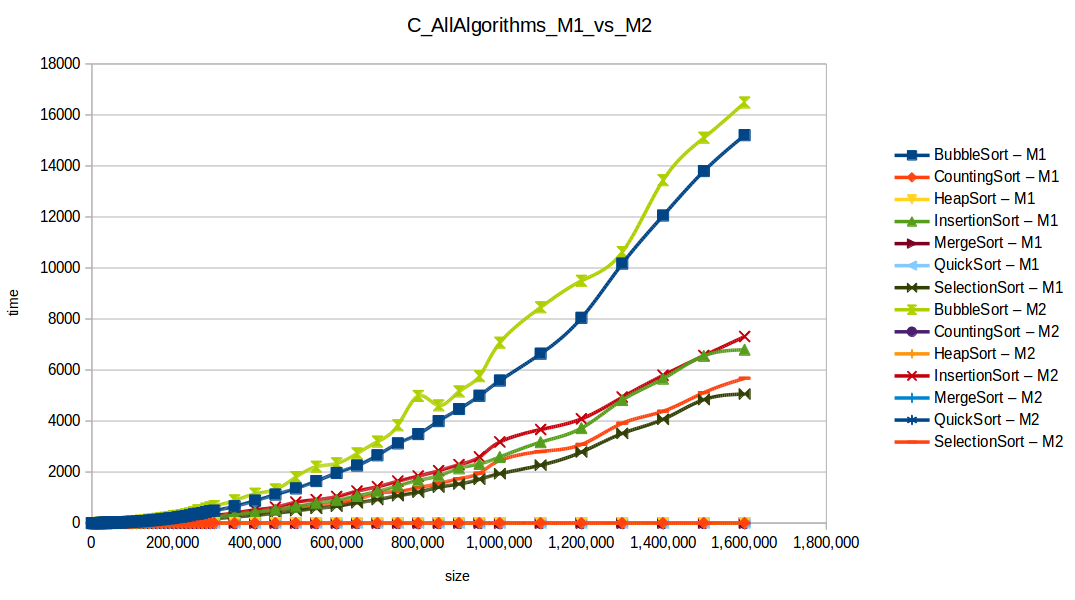
\includegraphics{./images/allAlgorithms_M1_M2.png}
\caption{GraficoComparación}
\end{figure}

\end{document}
